\section{Scheduling with Known Output Lengths: The WAIT Algorithm}
\label{sec:wait}

This section develops the \textit{Waiting for Accumulated Inference Threshold} (WAIT) algorithm for the case in which output lengths and arrival rates are known when thresholds are set. WAIT uses the fluid equilibrium from Section~\ref{sec:fluid} as a batching target: for each output-length class \(j\), it waits until enough prompts have accumulated before admitting a batch, so that the batch composition remains close to the equilibrium levels \(n_j^*\) across prefill and decode stages. This threshold structure is the key dimensionality reduction in the known-output-length case: instead of tracking every resident prompt's future KV-cache growth, the scheduler controls threshold-sized flows across prefill and decode stages. Under the corresponding memory feasibility condition, this rule prevents eviction cascades while allowing the server to approach the fluid throughput benchmark. The throughput guarantees below assume \(C \ge M^*\), where \(M^*\) is the memory requirement needed to support that fluid equilibrium in \eqref{eq:memory_multi2}; this is the stable or near-boundary regime in which the load-balanced equilibrium allocation across prefill and decode stages fits in memory. Section~\ref{sec:experiments} separately examines overloaded regimes, where the full offered-load benchmark is no longer feasible but the same load-balancing principle helps the scheduler use available capacity more effectively and reduce eviction-induced waste.

\subsection{Motivation: Why Naive Scheduling Fails}
\label{subsec:wait_motivation}

The condition \(C\ge M^*\) is a capacity condition, not a scheduling rule. It identifies when the fluid equilibrium can fit in memory, but it does not ensure that an online policy will keep work balanced across prefill and decode stages.

Consider a First-Come-First-Serve (FCFS) policy that admits prompts as soon as they arrive. Even when \(C=M^*\), so the fluid equilibrium fits exactly in memory, FCFS can move too much work into downstream decode stages and create a persistent throughput loss. The following proposition gives a worst-case lower bound for this failure mode.

\begin{proposition}\label{prop:lower_bound_FCFS}
When \(C=M^*\), there exists an instance in which First-Come-First-Serve (FCFS) incurs a throughput gap \(\throughput^* - \mathbb{E}[\throughput^{(T,\pi)}] = \Omega(1)\) as \(T \to \infty\).
\end{proposition}

The proof is provided in Appendix~\ref{appendix:proof_fcfs_lower_bound}. The example below is a simpler single-type illustration of the same eviction cascade.

\begin{example}[Eviction Cascade under FCFS]
\label{ex:fcfs_cascade}
Consider a single prompt type: a prompt such as ``Hello'' with a one-token response ``Hi,'' so \(l=1\) and \(l'=1\). Each prompt uses 1 unit of memory after prefill and 2 units after decode. Let \(C=12\) and \(\lambda=4\). The fluid equilibrium keeps 4 prompts at the prefill stage and 4 prompts at the decode stage, uses \(4 \times 1 + 4 \times 2 = 12\) units of memory, and completes 4 prompts per iteration.

Now suppose the system starts slightly imbalanced with 6 prompts at stage 0 (awaiting prefill) and 3 prompts at stage 1 (in decode). Under FCFS:
\begin{enumerate}
    \item \textbf{Iteration 1}: FCFS processes all 9 prompts. The 3 decode prompts complete, while the 6 prefill prompts advance to decode and require \(6 \times 2 = 12\) units of memory. The system is full after only 3 completions.
    \item \textbf{Iteration 2}: About 4 new prompts arrive during the previous iteration. Admitting them for prefill requires 4 additional memory units, so the server evicts 2 decode prompts to free \(2 \times 2 = 4\) units. The system returns to 4 prefill prompts and 4 decode prompts, again using \(4+8=12\) units.
    \item \textbf{Iteration 3}: The 4 decode prompts complete. The 2 evicted prompts have lost their KV caches and must restart from prefill, re-entering the queue alongside genuinely new arrivals. The restart mechanism perpetuates the imbalance.
\end{enumerate}
The eviction-restart cycle yields approximately 3--3.5 completions per iteration instead of the 4 completions sustained by the fluid equilibrium. Thus \(C=M^*=12\) is sufficient to support the fluid balance, but FCFS does not maintain that balance and loses effective throughput.
\end{example}

The operational implication is that having enough memory to support the fluid equilibrium does not by itself guarantee that the stochastic system will operate near that equilibrium. The scheduler must also regulate the composition of prompts across prefill and decode stages. FCFS admits prompts greedily, lets this composition drift away from the fluid balance, and thereby creates the eviction-restart cycle.

\subsection{The WAIT Algorithm}
\label{subsec:wait_algorithm}

The FCFS example points to the missing control variable: the composition of the in-service population across prefill and decode stages. WAIT regulates this composition by assigning each type \(j\) a threshold \(n_j\), interpreted as the target number of type-\(j\) prompts to serve from each prefill/decode stage in an iteration. If fewer than \(n_j\) new type-\(j\) prompts are waiting at entry, WAIT does not admit that type. Once the threshold is reached, the server processes up to \(n_j\) prompts from each prefill/decode stage of that type. In this way, new work enters the system only when it can replenish a balanced allocation across prefill and decode stages, rather than pushing the system toward the downstream buildup seen under FCFS.

The threshold rule also gives the analysis its tractable structure. Once the thresholds are fixed, each type evolves as a threshold queue observed at batch-completion epochs, while the shared memory interaction is captured by the feasibility of the threshold vector. The waiting requirement is therefore not merely a safety device against eviction; it also preserves the batching benefit created by the fixed overhead \(d_0\). Batches form at a scale large enough to use the server effectively, while the thresholds keep memory usage within capacity.

\paragraph{Algorithm Description.} For each prompt type \(j \in [m]\), WAIT sets a threshold \(n_j\) derived from the fluid model. At decision epoch \(t\), let \(n_{js}^t\) denote the number of type-\(j\) prompts at stage \(s\). Type \(j\) is eligible for the next batch only when
\[
n_{j0}^t \geq n_j.
\]
When this condition holds, WAIT selects \(\min\{n_j,n_{js}^t\}\) type-\(j\) prompts from each prefill/decode stage \(s\). If no type is eligible, the server waits for more arrivals. Prompts that are not selected remain in their current queues. A prompt waiting outside the GPU before prefill has no resident KV cache, but any prompt that has already been admitted and is waiting between decode iterations keeps its KV cache on the GPU and continues to count against memory. Algorithm~\ref{alg:wait} and Figure~\ref{fig:wait} describe the policy.

\begin{figure}
    \centering
    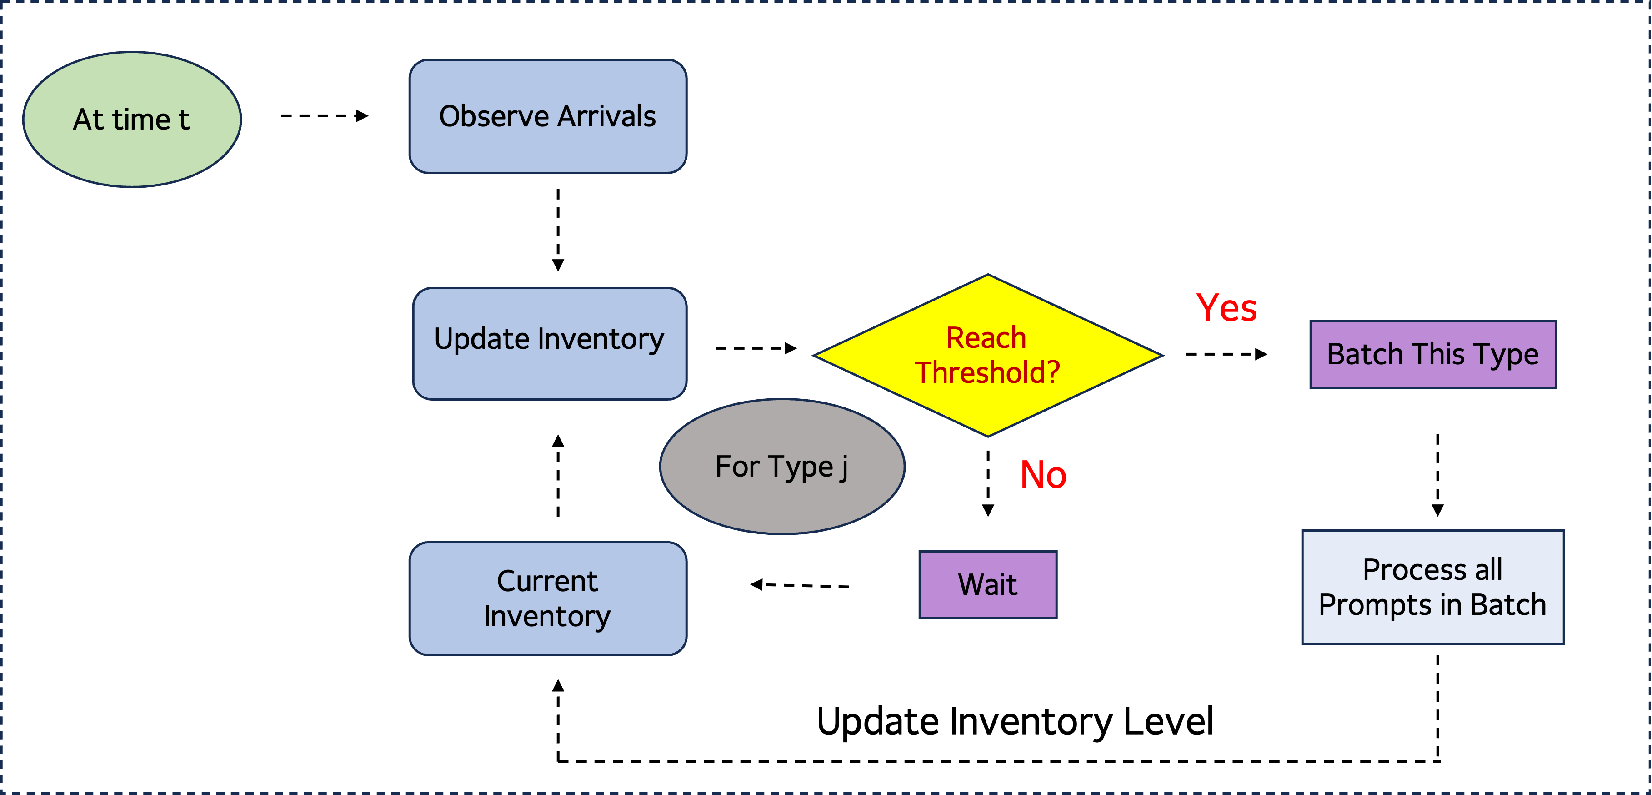
\includegraphics[width=0.85\linewidth]{Experiments_pdf/fig_WAIT.pdf}
    \caption{Batch formation under WAIT for a fixed type \(j\). The scheduler updates the type-\(j\) inventory and batches this type only when the prefill-entry queue reaches \(n_j\); otherwise, it waits and carries the inventory forward. When batched, up to \(n_j\) prompts from each prefill/decode stage are advanced.}
    \label{fig:wait}
\end{figure}

\begin{algorithm}[h]
\caption{WAIT: Waiting for Accumulated Inference Threshold}
\label{alg:wait}
{\small\linespread{1.0}\selectfont
\begin{algorithmic}[1]
\Require Memory $C$, arrival rates $\lambda_j$, thresholds $n_j$ satisfying \eqref{eq:wait_thresholds}, $\forall j \in [m]$
\State Initialize prompt inventory $n_{js} \gets 0$ for all $j \in [m], s \in \{0, 1, \dots, l_j'\}$
\State Initialize event queue with arrival events for each type $j$
\State Set current time $t \gets 0$
\State Set server status to idle
\While{True}
    \State Wait for the next event (arrival or batch completion)
    \If{event is an arrival of type $j$}
        \State Update inventory: $n_{j0} \gets n_{j0} + 1$  \Comment{Add new prompt to waiting queue of prefill phase}
    \ElsIf{event is a batch completion}
        \State Retrieve the selected counts $a_{js}$ stored with the completed batch
        \State Simultaneously advance selected prompts one stage: $n_{js}\gets n_{js}-a_{js}$ and $n_{j,s+1}\gets n_{j,s+1}+a_{js}$ for $s<l_j'$
        \State Clear KV caches for the $a_{j,l_j'}$ prompts completing after stage $l_j'$  \Comment{Free memory for completed prompts}
        \State Set server status to idle
    \EndIf
    \State Set \(J(t)\gets\{j\in[m]: n_{j0}\ge n_j\}\)  \Comment{Eligible types}
    \If{server is idle and \(J(t)\neq\emptyset\)}
        \State For every \(j\in J(t)\) and stage \(s\), set \(a_{js}\gets\min\{n_j,n_{js}\}\)
        \State Form batch \(B\) from all selected prompts and store \(a_{js}\) with \(B\)
        \State Process batch $B$; keep already resident prompts outside the batch waiting with their KV caches retained
        \State Set server status to busy until the completion event for \(B\)
    \EndIf
\EndWhile
\end{algorithmic}
}
\end{algorithm}

\subsection{Asymptotic Guarantees}
\label{subsec:asymptotic_analysis}
\label{subsec:main_theorem}
We analyze WAIT in an asymptotic scaling that averages out stochastic fluctuations while preserving the fixed memory constraint. For \(\zeta\ge 1\), arrival rates scale as \(\lambda_j^{(\zeta)}=\zeta\lambda_j\) and processing times scale as \((d_0^{(\zeta)},d_1^{(\zeta)})=(\zeta^{-1}d_0,\zeta^{-1}d_1)\), with memory capacity \(C\) fixed. For WAIT, the required physical memory is \(M_{\mathrm{req}}^{(\zeta,\pi)}=M^\pi\), which is independent of \(\zeta\) because no downstream boundary buffer is needed. For a policy \(\pi\), let \(N_j^{(\zeta,\pi)}\) be the number of completed decode tokens from type-\(j\) prompts over this horizon, and define
\[
\throughput^{(\zeta, \pi)} = \frac{1}{\zeta T} \sum_{j=1}^m N_j^{(\zeta, \pi)}.
\]
For delay metrics, let \(\Latency_{\rm cal}^{(\zeta,\pi)}\) and \(\TTFT_{\rm cal}^{(\zeta,\pi)}\) denote the elapsed calendar-time averages over this scaled system. The theorem reports the service-normalized delays \(\Latency^{(\zeta,\pi)}:=\zeta\Latency_{\rm cal}^{(\zeta,\pi)}\) and \(\TTFT^{(\zeta,\pi)}:=\zeta\TTFT_{\rm cal}^{(\zeta,\pi)}\), so the effective horizon in the bounds is \(\zeta T\). The benchmark is the fluid throughput \(\throughput^*=\sum_{j=1}^m \lambda_j l_j'\) in \eqref{throughput_fluid_multiple}.

Assume \(C \ge M^*\), with \(M^*\) given by \eqref{eq:memory_multi2}. Consider a WAIT policy \(\pi=[n_1,\dots,n_m]\), where \(n_j\) is the type-\(j\) threshold applied at each prefill/decode stage. The threshold vector must satisfy a load-balance condition and a memory condition:
\begin{equation}
\label{eq:wait_thresholds}
\begin{aligned}
\Delta T(n_{1:m}) &:= d_0 + d_1 M^{\pi} \leq \tfrac{n_j}{\lambda_j},\, \forall j\in[m],\\
 M^{\pi} &= \sum_{j=1}^m n_j (l_j' + 1) \big(l_j + \tfrac{l_j'}{2}\big),\\
 M^* &\leq M_{\mathrm{req}}^{(\zeta,\pi)}:=M^\pi \leq C
\end{aligned}
\end{equation}
The first line is the arrival-completion balance for each type: during an iteration of length \(\Delta T(n_{1:m})\), the expected number of type-\(j\) arrivals is \(\lambda_j\Delta T(n_{1:m})\), and WAIT serves \(n_j\) type-\(j\) prompts from each active stage. The memory condition then asks the threshold vector to be large enough to support the fluid equilibrium, but not so large that the required memory \(M_{\mathrm{req}}^{(\zeta,\pi)}\) exceeds the available physical capacity \(C\). The condition \(M^*\le C\) says that the workload is stabilizable in the fluid model; the theorem below shows that WAIT realizes this stability in the stochastic system by keeping memory growth under control.

\begin{theorem}
\label{thm:wait_heavy_traffic}
If the thresholds \(\pi=[n_1,\dots,n_m]\) satisfy \eqref{eq:wait_thresholds}, then
\[
\begin{aligned}
&\throughput^*-\ex{}{\throughput^{(\zeta,\pi)}}=O((\zeta T)^{-\frac{1}{2}}),\\
&\ex{}{\Latency^{(\zeta,\pi)}},\,\ex{}{\TTFT^{(\zeta,\pi)}}=O\prn{(\zeta T)^{\frac{1}{2}}}.
\end{aligned}
\]
Moreover, if \(\Delta T(n_{1:m})<n_j/\lambda_j\) for all \(j\in[m]\), then
\[
\begin{aligned}
&\throughput^* - \ex{}{\throughput^{(\zeta,\pi)}} = O(1/(\zeta T)), \\
&\ex{}{\Latency^{(\zeta,\pi)}},\, \ex{}{\TTFT^{(\zeta,\pi)}} = O(1).
\end{aligned}
\]
\end{theorem}

The theorem rests on the control structure created by WAIT. The difficult step is not to prove recurrence after a stable queue has been isolated. Instead, it is to design a batching rule that keeps endogenous KV-cache growth under control before memory overflows. Each admitted prompt creates a KV cache that grows throughout decode. If an unstructured batching rule admits too much work, these caches can exceed memory in later iterations, forcing eviction and restart. The restarted prompts then return as future work and can reduce effective throughput even when the fluid memory requirement fits within capacity. WAIT prevents this failure mode by fixing a target allocation across prefill and decode stages through \(n_{1:m}\). Given this threshold vector, every full batch has memory usage \(M^\pi\) and iteration length \(\Delta T(n_{1:m})\), and the main stochastic component for type \(j\) is the time until its entry queue reaches \(n_j\). The proof uses the threshold structure to define an auxiliary embedded full-threshold process observed at review epochs and then couples it to the event-driven WAIT sample path type by type: although realized WAIT batches may contain different subsets of eligible types, each type's threshold batch receives a corresponding service opportunity within one full-threshold review interval. This coupling turns the original memory-coupled controlled process into threshold queues tied together by the deterministic feasibility condition \(M^\pi\le C\). The complete proof is in Appendix~\ref{appexidx::proof of wait_heavy_traffic}.

The square-root delay bound at the boundary is also unavoidable among policies that keep up with the fluid throughput benchmark. When the threshold queues have no slack, their fluctuations cannot be averaged away by any non-predictive online rule, even if the total memory equals the fluid memory requirement. The next proposition gives the matching lower bound for latency and TTFT.
\begin{proposition}\label{prop::simple random walk, tight bound}
There exists an instance where \( C = M^* \), and for any non-predictive online policy \(\pi\) whose normalized effective-throughput gap is \(o(1)\), the expected average latency and TTFT satisfy
\[
\mathbb{E}[\Latency^{(\zeta,\pi)}],\quad \mathbb{E}[\TTFT^{(\zeta,\pi)}] = \Omega((\zeta T)^{1/2}).
\]
\end{proposition}
The strict inequalities in Theorem~\ref{thm:wait_heavy_traffic} correspond to slack in these threshold queues. If \(\Delta T(n_{1:m})<n_j/\lambda_j\), the type-\(j\) entry queue has negative drift, and the average latency and TTFT of type-\(j\) prompts remain \(O(1)\).

The policy in this section assumes that output lengths and arrival rates are known when the thresholds are set. In practice, these quantities can be estimated from predictors \citep{fu2025efficient}, but an online serving system may not know a request's decode length at admission. The next section relaxes this information requirement by developing a nested version of WAIT for unknown output lengths.
